\subsection{Heur\'istica constructiva Golosa}

Una heur\'istica constructiva golosa es una que va armando la soluci\'on tomando, en cada paso, la mejor decisi\'on local; es decir la que conviene en ese momento, sin tener en cuenta las posibles consecuencias que esa decisi\'on puede tener en los pasos futuros.\\

\subsection{Descripci\'on del algoritmo}

Para resolver el problema mediante una heur\'istica golosa elegimos el enfoque constructivo; es decir, en el cual la soluci\'on se genera tomando la mejor elecci\'on local a cada paso.\\\\

Inicialmente el algoritmo obtiene los caminos m\'inimos entre $u$ y $v$ tanto en $w_1$ como en $w_2$ utilizando el algoritmo de Floyd, el cual nos da adem\'as todos los caminos m\'inimos entre todos los nodos (todos a todos).\\
Llamaremos a partir de ahora $c_1$ al camino m\'inimo entre $u$ y $v$ en $w_1$ y $c_2$ al camino m\'inimo entre los mismos nodos pero en $w_2$.\\
Una vez obtenidos $c_1$ y $c_2$ verificamos que el peso de $c_1$ est\'e acotado por $K$ con respecto a $w_1$; caso contrario, no hay soluci\'on.\\
Pasada esta verificaci\'on, y si $c_2$ no est\'a acotado por $K$ (en cuyo caso ya tendr\'iamos una soluci\'on exacta) el algoritmo procede a ir armando el camino soluci\'on. Al ser una heur\'istica golosa constructiva, va a ir armando el camino insertando de a un nodo a la vez y tomando la mejor decisi\'on posible para el nodo que est\'a analizando en cada iteraci\'on, llamado $nodo\_actual$ en el algoritmo. 
El criterio de elecci\'on del pr\'oximo nodo es el siguiente: 

\begin{itemize}
\item Comienza tomando como $nodo\_actual$ al nodo source, en nuestro caso $u$.
\item Inserta en el camino soluci\'on al $nodo\_actual$.
\item Aqu\'i es donde analiza las posibles opciones locales y toma la mejor opci\'on posible a su alcance:
\item Como primera medida obtiene un camino m\'inimo con respecto a $w_2$ desde el $nodo\_actual$ hasta el target, llamemoslo $c2\_{potencial}$, y corrobora que tenga peso menor a $K$ con respecto a $w_1$. De ser as\'i ser\'a la mejor soluci\'on que podr\'a obtener mediante esta heur\'istica por lo tanto retornar\'a el camino constru\'ido al momento unido al $c2\_{potencial}$.
\item Caso contrario corrobora si, desde el primer nodo del $c2\_{potencial}$, llamemoslo $nodo1\_c2$, construyendo un camino m\'inimo hasta $v$ en relaci\'on a $w_1$, se puede llegar a obtener una soluci\'on v\'alida, en este caso marca como $nodo\_actual$ a $nodo1\_c2$ y vuelva a realizar el mismo procesamiento.
\item En el caso de que el \'ultimo item no sea posible, corroborar\'a si desde el $nodo\_actual$ a\'un se puede construir un camino m\'inimo en $w_1$ hasta $v$, es decir, que no supere la cota $K$. Para ello construye un camino m\'inimo, $c1\_{potencial}$, desde $nodo\_actual$ hasta el target para $w1$ y en caso que el peso sea v\'alido coloca como $nodo\_actual$ al primer nodo del $c1\_{potencial}$ y vuelve a iterar. Caso contrario llega a una situaci\'on en la cual no podr\'a encontrar una posible soluci\'on y debe terminar.
\end{itemize}

Veamos entonces la componente greedy de la heur\'istica. Como mencionamos previamente el algoritmo es constructivo por ende en cada iteraci\'on se para en un nodo y all\'i tiene tres posibles opciones para seguir construyendo la soluci\'on. Las mismas son completamente locales, es decir, no tiene una visi\'on general, sino que se limita a escoger la mejor opci\'on (el siguiente nodo a incorporar en nuestra soluci\'on constructiva) dentro de los primeros nodos dados por los caminos m\'inimos para $w_1$ y $w_2$, y asume que de esta manera podr\'a ir construyendo una soluci\'on factible.

%Analicemoslo mejor mediante un diagrama de flujo:

\subsubsection{Diagrama de flujo}
\begin{figure}[!hp]
	\centering
 	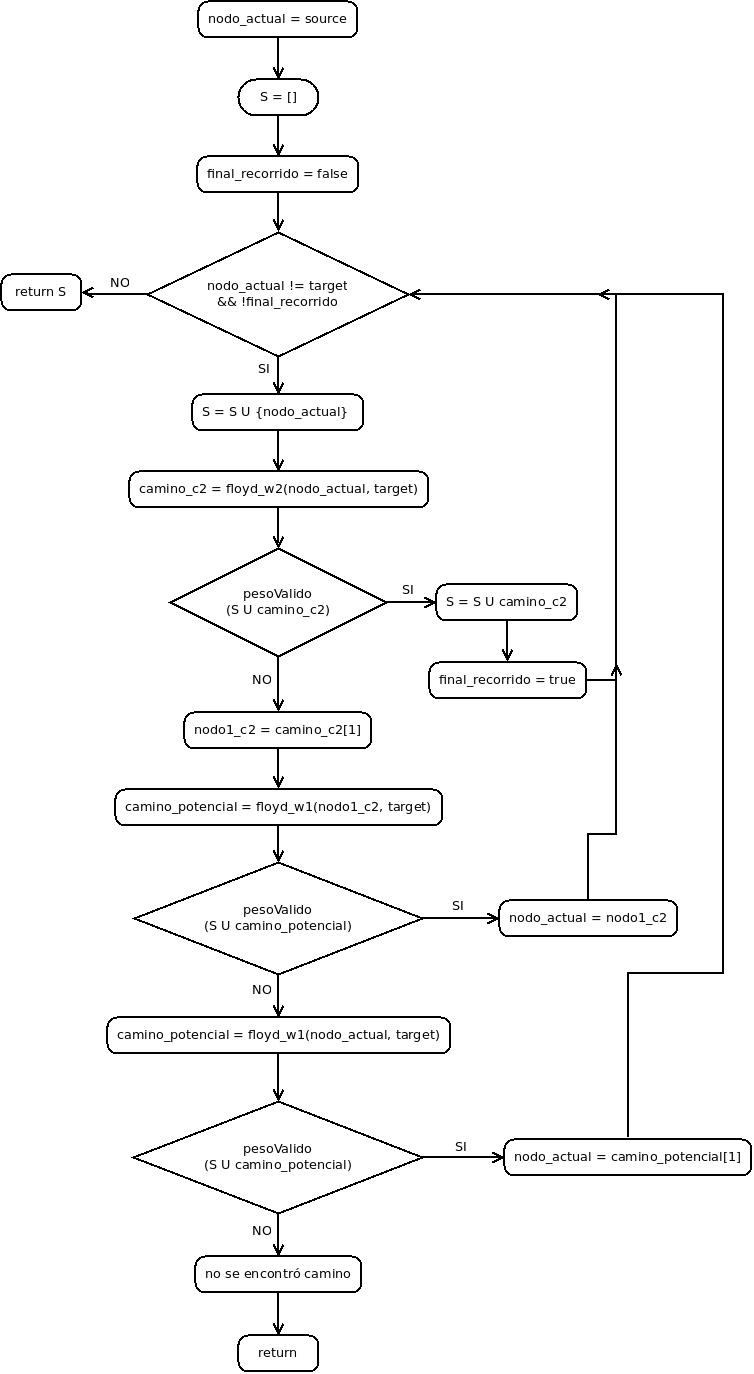
\includegraphics[height=\textheight]{img/flujo_greedy.jpeg}
\end{figure}

%\newpage


\newpage
\subsection{Algoritmo}
\lstset{language=C++,
                basicstyle=\ttfamily\footnotesize,
                keywordstyle=\color{blue}\ttfamily,
                stringstyle=\color{red}\ttfamily,
                commentstyle=\color{green}\ttfamily,
                morecomment=[l][\color{magenta}]{\#},
                breaklines=true
}
\begin{lstlisting}

void heuristicaGreedy::execute(graph * grafo) {

	vector<vector<double> > pesos1_orig = grafo->get_weights1();
	vector<vector<double> > pesos2_orig = grafo->get_weights2();

	vector<vector<double> > pesos1 = grafo->get_weights1();
	vector<vector<double> > pesos2 = grafo->get_weights2();
	Algoritmos* algoritmo = new Algoritmos();

	vector<vector<int> > floyd1 = algoritmo->floyd(pesos1);
	vector<vector<int> > floyd2 = algoritmo->floyd(pesos2);
	

	/* Si el camino minimo en w1 es mayor a la cota K entonces no hay solucion */
	vector<int> camino_w1 = algoritmo->reconstruirPathFloyd(u, v, floyd1);
	if(!pesoEnRegla(camino_w1, pesos1_orig)) {
		cout << "no" << endl;
		return;
	}

	/* Si el camino minimo en w2 respeta la cota K entonces es la solucion exacta */
	vector<int> camino_w2 = algoritmo->reconstruirPathFloyd(u, v, floyd2);
	if(pesoEnRegla(camino_w1, pesos1_orig)) {
		imprimirSolucion(camino_w2, pesos1_orig, pesos2_orig);
		delete algoritmo;
		return;
	}

	unsigned int nodoActual = u;
	bool finalRecorrido = false;
	vector<int> caminoFinal = vector<int>();
	while(nodoActual != v && !finalRecorrido) {
		caminoFinal.push_back(nodoActual);
		camino_w2 = algoritmo->reconstruirPathFloyd(nodoActual, v, floyd2);

		/* tomo el primer nodo nodo_1 del camino_w2 entre el nodoActual y v, 
			- caso 1: si es menor a k el peso en w1 entonces es el minimo posible por aca en w2 y cumple w1 
		 	- caso 2: sino me fijo si en el peor de los casos, siguiendo por nodo_1 y a partir de ahi hacer
		 		el camino_w1 cumple que el peso sea menor a k, si es asi avanzo un nodo y repito el procedimiento
		 	- caso 3: si ninguna de las dos condiciones anteriores se cumple entonces me veo obligado a avanzar al
		 		primer nodo del camino_w1 y repetir el procedimiento */

		/* primer nodo del camino_w2 */
		int nodo1_w2 = camino_w2[1];
		vector<int> camino_w2_potencial = algoritmo->reconstruirPathFloyd(nodo1_w2, v, floyd2);
		vector<int> camino_aux = unirCaminos(caminoFinal, camino_w2_potencial);
		camino_aux.push_back(v);

		if(pesoEnRegla(camino_aux, pesos1_orig)) {
			/* caso 1 */
			caminoFinal = unirCaminos(caminoFinal, camino_w2_potencial);
			finalRecorrido = true;
		} else {
			/* caso 2 o 3 */
			vector<int> camino_w1_potencial = algoritmo->reconstruirPathFloyd(nodo1_w2, v, floyd1);
			vector<int> camino_aux = unirCaminos(caminoFinal, camino_w1_potencial);
			camino_aux.push_back(v);
			if(pesoEnRegla(camino_aux, pesos1_orig)) {
				/* caso 2 */
				nodoActual = nodo1_w2;
			} else {
				camino_w1_potencial = algoritmo->reconstruirPathFloyd(nodoActual, v, floyd1);
				vector<int> camino_aux = unirCaminos(caminoFinal, camino_w1_potencial);
				camino_aux.push_back(v);
				if(pesoEnRegla(camino_aux, pesos1)) {
					/* primer nodo del camino_w1 */
					nodoActual = camino_w1_potencial[1]; 				
				} else {
					cout << "no";
					return;
				}
			}
			
		}
	}

	/* por ultimo agregamos v al camino final */
	caminoFinal.push_back(v);

	imprimirSolucion(caminoFinal, pesos1_orig, pesos2_orig);
	
	delete algoritmo;
	
	return;
	
}

vector<int> heuristicaGreedy::unirCaminos(vector<int> camino1, vector<int> camino2) {
	int size1 = camino1.size();
	int size2 = camino2.size();
	vector<int> caminoNuevo = vector<int>(size1 + size2 - 1, 0);
	
	for(int i=0; i<size1; i++) {
		caminoNuevo[i] = camino1[i];
	}

	for(int i=0; i<size2 - 1; i++) {
		caminoNuevo[size1 + i] = camino2[i];
	}

	return caminoNuevo;
}

\end{lstlisting}


\newpage
\subsection{Familia de grafos sin soluci\'on \'optima}
Dado que la her\'istica es golosa constructiva, en cada paso se quedar\'a con la mejor opci\'on posible para poder continuar armando la soluci\'on. En nuestro caso la mejor opci\'on posible comienza siendo el camino m\'inimo en $w_2$ desde el $nodo\_actual$ hasta $v$, luego pasa por seguir iterando desde el primer nodo del camino m\'inimo desde el primer nodo del camino anterior hasta el target en $w_1$ y sino, de ser posible, se queda con el primer nodo del camino m\'inimo desde el $nodo\_actual$ hasta $v$. 
Como podemos ver nuestra elecci\'on est\'a limitada a los primeros nodos pertenecientes a los caminos m\'inimos en $w_1$ y $w_2$. Por lo tanto podr\'iamos identificar la siguiente familia para la cual podr\'ia no retornar una soluci\'on \'optima o ni siquiera encontrar alguna:

\begin{itemize}
\item Como mencionamos previamente, la elecci\'on del siguiente nodo a analizar esta limitada a nodos de los caminos m\'inimos, por ende si la soluc\'on \'optima $S$ se encontrara completamente fuera de las opciones analizadas no habr\'ia forma de hallarla. Es decir, si $S$ pasara por un nodo $v_i$ adyacente al $nodo\_actual$, y que el mismo no sea ninguno de los candidatos que se analizan en cada iteraci\'on, entonces no tendr\'iamos forma de poder encontrar $S$. 
Para esta familia de grafos, no podr\'amos estimar de antemano que tan mala puede llegar a ser la soluci\'on encontrada. Es m\'as, hasta podr\'amos no encontrar ninguna en casos donde si era posible hallarla.
\begin{figure}[!hp]
	\centering
 	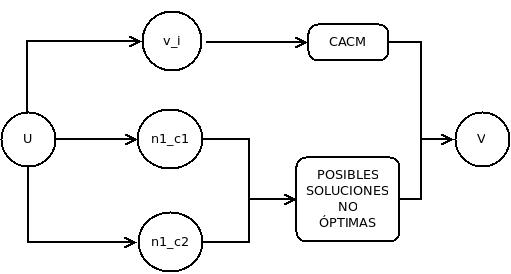
\includegraphics[scale=0.6]{img/familia_greedy.jpeg}
\end{figure}
\end{itemize}


\newpage
\subsection{An\'alisis de complejidad}
Para el an\'alisis de complejidad separaremos el algoritmo en tres tramos:
\begin{itemize}
\item Generaci\'on de caminos m\'inimos mediante el algoritmo de Floyd:
	Antes de comenzar a construir la soluci\'on debemos contar con los caminos m\'inimos de todos los nodos contra todos los dem\'as, tanto para el peso $w_1$ como para $w_2$. Es por eso que para esta tarea utilizamos el algoritmo de Floyd, cuya complejidad es O($n^3$). 
\item Validaci\'on de casos borde:
	Antes de comenzar a armar el camino corroboramos que pueda llegar a existir una soluci\'on, para esto reconstru\'imos el camino de $u$ a $v$ en $w_1$ y vemos que no supere la cota $K$. 
	Lo mismo hacemos para la mejor soluci\'on, si al reconstruir el camino en $w_2$ tenemos un camino que respeta la cota indicada, entonces tenemos la mejor soluci\'on, por ende no es necesario seguir con el procesamiento.
	En ambos casos utilizamos dos funciones auxiliares:
	\begin{itemize}
	\item reconstruirPathFloyd: Documentada en el c\'odigo con complejidad de peor caso O($n$).
	\item pesoEnRegla: Documentada en el c\'odigo con complejidad de peor caso O($n$).
	\end{itemize}
\item Construcci\'on de la soluci\'on:
	En este tramo vamos a ir armando el camino realizando a lo sumo n iteraciones, caso en el que tendr\'iamos un camino hamiltoniano que pasa por todos los nodos. Por ende, habr\'ia que ver que pasa en cada iteraci\'on y as\'i poder evaluar la complejidad del tramo completo.
	Para esta parte tambi\'en se utiliza la funci\'on $unirCaminos$ cuya complejidad del peor caso es O($n^2$).
	Si analizamos el c\'odigo podremos notar que se utilizan por separado las 3 funciones mencionadas al momento, por lo tanto para obtener la complejidad de este tramo tendr\'iamos que "anidar" la mayor complejidad dentro de cada iteraci\'on a la cantidad de iteraciones realizadas. En este caso ser\'ian $n$ iteraciones con complejidad O($n^2$) cada una, obteniendo una complejidad total del peor caso de este tramo de O($n^3$).
\end{itemize}

Acabamos de analizar las complejidades de 3 tramos del algoritmo que se ejecutan de manera separada, por ende si sumamos sus complejidades, O($n^3$) + O($n$) + O($n^3$), vemos que la complejidad total del peor caso de la heur\'istica es O($n^3$).

